\spaltenanfang
Herzlich willkommen bei uns am Fachbereich! Was du gerade in deinen Händen
hältst, ist die Zeitschrift der diessemestrigen Orientierungsveranstaltung, die
wir „Don’t Panic“ getauft haben. \textbf{Don’t Panic!} - das soll auch als
Motto über der ganzen Veranstaltung stehen.


Es ist mal wieder April, und es haben sich 200 Menschen entschlossen,
in Frankfurt einen Studiengang der Informatik aufzunehmen. Darunter sind
Einige, die schon vorher etwas anderes studiert haben oder von einer anderen
Hochschule kommen. Die kennen sich meist schon recht gut im Uni-Dschungel aus,
und auch die ganzen Begriffe, Abkürzungen und Redewendungen sind für sie keine
böhmischen Dörfer mehr. Aber für einen beachtlichen Teil der Erstsemester ist
erfahrungsgemäß so ziemlich alles neu. Und deswegen werden wir uns bemühen,
euch während dieser Orientierungsveranstaltung so ziemlich alles zu erklären.
Ihr werdet hoffentlich schnell merken, dass das alles halb so wild ist und kein
Grund zur Panik besteht, also \textbf{Don’t Panic}! Bei dieser
Orientierungsveranstaltung haben wir uns im Wesentlichen zwei Ziele gesetzt:


Wir wollen euch mit allen notwendigen Informationen versorgen, damit ihr an
eurem ersten Tag in der Uni wenigstens so ungefähr wisst, wo die wichtigsten
Einrichtungen sind, welche Veranstaltungen so laufen und welche davon für euch
Sinn machen. Wir wollen euch ein paar Ratschläge und Tipps mit auf den Weg
geben, und nicht zuletzt können wir euch von einer großen Sammlung von Fehlern
berichten, die wir gemacht haben und die \textsl{ihr} ja nicht unbedingt noch
mal machen müsst.


Das Uni-Leben und das Informatik-Studium bringen viele Begriffe mit sich, die
euch vielleicht unbekannt sind. Vielleicht möchtet ihr einige Stichworte auch
noch einmal in kompakter Form nachlesen. Aus diesem Grund haben wir euch ab
Seite \pageref{glossar} ein Glossar der wichtigsten Begriffe zusammengestellt.


Aber wir möchten auch, dass ihr euch heute gegenseitig ein
bisschen kennenlernt, damit euch am nächsten Montag wenigstens schon ein paar
Gesichter bekannt vorkommen, wenn der Stress losgeht. Ganz generell empfehlen
wir, sich in kleinen Gruppen zusammenzutun. In einer Gruppe weiß eigentlich
immer jemand, was wo aushängt, bis wann man sich irgendwo eingetragen haben
muss und Vieles mehr. Auch das eigentliche Studieren, das Lernen und das Lösen
von Aufgaben ist in einer Gruppe wesentlich erfolgversprechender und mit
Sicherheit angenehmer.\\
\spaltenende
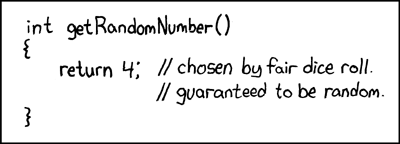
\includegraphics{comics/random_number}
